\chapter[Produtos, Atividades e Cronograma]{Produtos, Atividades e Cronograma}

\section{Resumo da proposta}
\section{Estrutura Analítica do Projeto}

A figura a seguir mostra a estrutura analítica do projeto. O projeto foi dividido em 3 fases: Iniciação, cujo objetivo é obter a viabilidade e a construir o referencial teórico do projeto; Construção, cujo objetivo é realizar de fato as atividades de testes e análise estática; e Transição, cujo objetivo é entregar a integração contínua e finalizar o projeto.

\begin{figure}[h]
 \centering
 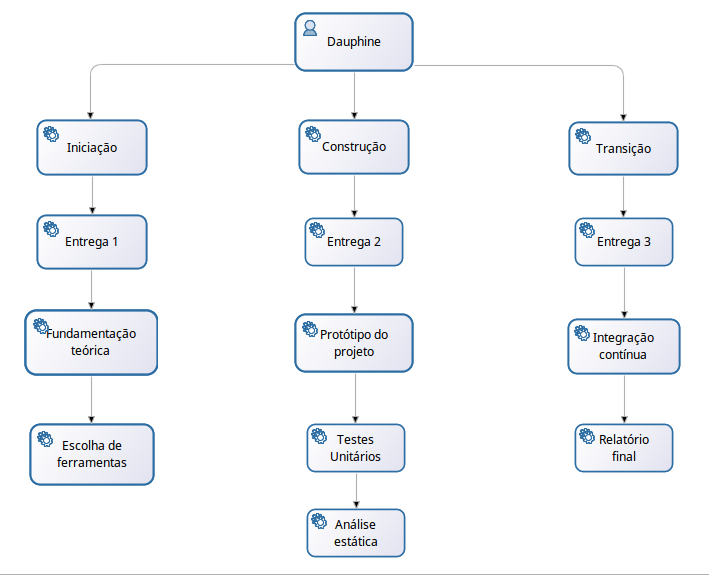
\includegraphics[width=3cm, height=4cm]{figuras/eap.png}
 \caption{Estrutura Analítica do Projeto}
\end{figure}

\section{Lista de Software}
\section{Cronograma de Atividades}
